%\documentclass[a4paper,11pt,twocolumn]{article}
\documentclass[a4paper,11pt]{article}

\usepackage[utf8]{inputenc}
\usepackage[french]{babel}
\usepackage{graphicx}
\usepackage{xcolor}
\usepackage{listings}
\usepackage{geometry}
\geometry{
	top=1in,
	inner=1in,
	outer=1in,
	bottom=1in,
	headheight=3ex,
	headsep=5ex,
}
%\usepackage{fullpage}
\usepackage{fancyhdr}
\lhead{m@j4.pe}
\rhead{Privatiser vos mails}
\pagestyle{fancy}

\setlength\parindent{0em}

%\setlength\parindent{0em} % pas d'indetn de patagraph
\title{Privatiser vos mails\\via\\OpenBSD/OpenSMTPD}
\author{m@j4.pe}
\date{\today}

 
\begin{document}

\maketitle

\abstract 

Je pars du principe que vous avez un serveur de VMs KVM avec des IPFO. Je suis
chez Online.net, j'ai un R220v1.\\
L'article décrit comment installer un serveur de mail {\bf simple} perso/famille 
qui ne demande pas une grosse gestion des utilisateurs.
Cet article suivra le schéma suivant :\\
\begin{itemize}
	\item Installation d'une VM OpenBSD sur un serveur KVM - GNU/Linux Debian
	\item Mise en place de OpenSMTPd comme serveur SMTP
	\item Mise en place d'un serveur DovCot comme serveur Imap
	\item Un peu de pf
\end{itemize} 
\vspace{5mm}
Enfin, les sources de cet article sont disponibles via un SCM\footnote{http://github.com/j4/articles/}. 
Merci de contribuer si vous souhaitez le compléter.

\section*{Installation d'une VM avec Linux/Kvm et virt-install}

Nous allons installer une VM avec deux cartes réseaux et deux disques durs. Une
carte réseau sur un réseau interne au serveur de VM (réseau d'administration)
et une carte réseau qui se trouve sur l' internet. Les deux disques durs sont
le disque dur de l'os (10G) et le disque dur des data dimensionés à la taille
de vos boîtes mails.\\
J'utilise "virt-install" pour créer des vm. Voici la commande que j'utilise :

\vspace{5mm}
\begin{lstlisting}[language=bash,caption={Création d'une VM OpenBSD avec KVM},frame=bt,breaklines=true]
virt-install 
--connect=qemu:///system 
-n $SERVERNAME -r 2048 --vcpus=1 
-c iso/cd53.iso 
--disk /var/lib/libvirt/images/$SERVERNAME.img,size=10 
--disk /var/lib/libvirt/images/$SERVERNAME.data.img,size=$DATASIZE 
--network bridge=br0,model=e1000,mac=$MACADDR --network 
model=e1000,network=default 
--vnc -k fr --autostart
\end{lstlisting}
\vspace{5mm}
\begin{itemize}
	\item {\bf \$SERVERNAME} est le nom du serveur
	\item {\bf \$MACADDR} est l'addresse MAC fournie par votre hoster (cf les docs ipfo de
celui-ci)
	\item {\bf \$DATASIZE} est la taille de votre disque qui contiendra les datas/mails
\end{itemize}

Une fois la commande executée, il faut ce connecter via VNC à la console du
serveur afin de faire l'installation. X étapes :\\

\begin{itemize}
	\item Trouver le port vnc de la vm via virsh
	\item Port forwarding du port vnc afin de se connecter depuis notre poste client
	\item Installation depuis la console vnc
\end{itemize}

\vspace{5mm}
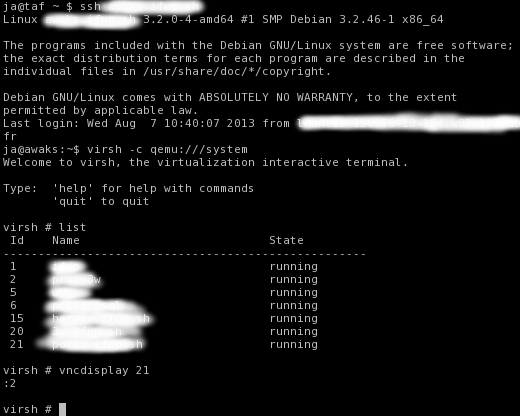
\includegraphics[scale=0.70]{medias/vncdisplay.png}
\vspace{5mm}

Maintenant que je connais le port (:2) de la console VNC de la VM je peux finir
l'installation en faisant un port forwarding sur celui-ci. Tu peux utiliser virt-manager mais comme ta
machine cliente est *BSD tu fais autrement.

\vspace{5mm}
\begin{lstlisting}[language=bash,caption={Création d'une VM OpenBSD avec KVM},frame=bt,breaklines=true]
ssh -L5902:127.0.0.1:5902 monserveur.devms.fr
\end{lstlisting}

\vspace{5mm}
puis depuis mon client :

\vspace{5mm}
\begin{lstlisting}[language=bash,caption={Création d'une VM OpenBSD avec KVM},frame=bt,breaklines=true]
vnclient 127.0.0.1:5902
\end{lstlisting}

\vspace{5mm}
\section*{Installation d' OpenBSD}

Le disque qui contient les data (boites mail) est {\bf chiffré} en utilisant la
méthode raid0 chiffrée d'OpenBSD. 

\vspace{5mm}
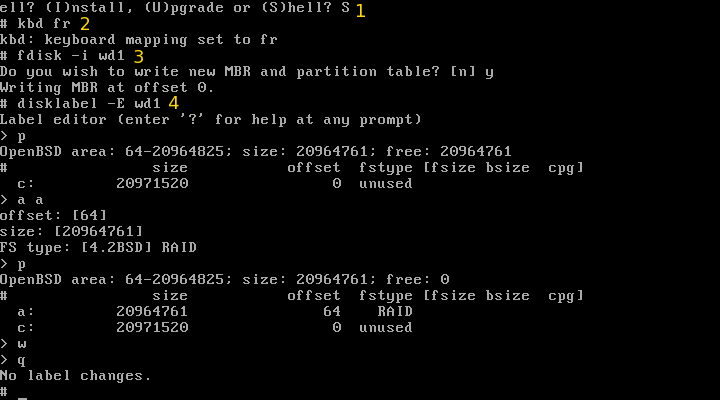
\includegraphics[scale=0.70]{medias/prepadisk.png}
\vspace{5mm}

\begin{itemize}
	\item Je n'installe pas encore car il faut que je mette en place le raid0 chiffrée
 avant de passer à l'install. Je passe donc en mode shell. 
	\item Je passe le clavier en fr
	\item fdisk pour init le mbr du dique qui contiendra le raid0
	\item disklabel, création d'une partoche RAID !
\end{itemize}

\vspace{5mm}
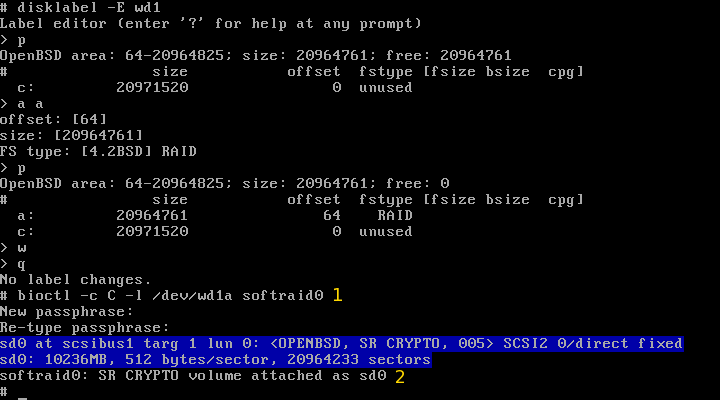
\includegraphics[scale=0.70]{medias/bioctl.png}
\vspace{5mm}

\begin{itemize}
	\item Création d'un softraid0 chiffré sur la partoche que nous avons créée
plus tôt. cf man bioctl
	\item Noter bien le nom du nouveau disque pour l'utiliser plus tard dans
 l'installation. (sd0 dans notre cas).
\end{itemize}

\vspace{5mm}
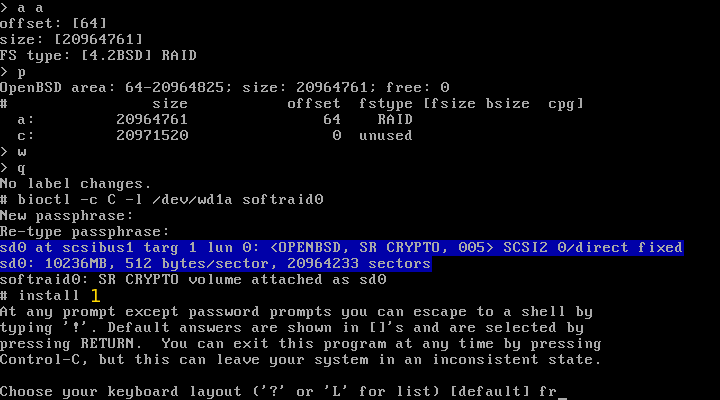
\includegraphics[scale=0.70]{medias/install.png}
\vspace{5mm}

Puis installation classique d'OpenBSD. Pour ma part, j'utilise le réseau
interne "administration" pour faire l'installation (em1 dans notre cas). 
Je configure l'ipfo plustard.\\
Attention à bien créer les partitions sur le disque raid0 chiffré qui à été crée. Par exemple
{\bf sd0a}.

\section*{Configuration du serveur}

Maintenant que nous avons une distrib toute fraîche, nous allons la configurer
afin d'utiliser l'ipfo.

\vspace{5mm}
\begin{lstlisting}[language=bash,caption={Config. du serveur},frame=bt,breaklines=true]
$ cd /etc/
$ cat hostname.em1
inet 10.73.0.100
$ cat hostname.em0
inet 88.190.xxx.xxx 255.255.255.255 # Mettre votre ipfo
!route add -inet 88.190.16.1/32 -link -iface em0 # A adapter suivant votre
ipfo
$ cat resolv.conf
nameserver 10.73.0.1
nameserver 8.8.4.4 
$ cat mygate
88.190.16.1 # A adapter suivant votre ipfo
\end{lstlisting}

\vspace{5mm}
Montage de la partition chiffrée au boot. Cela implique d'avoir une console VNC
si vous devez rebooter/booter la VM.

Editer le fichier {\bf /etc/rc.local} et ajouter le code suivant :

\vspace{5mm}
\begin{lstlisting}[language=bash,caption={Montage partition chiffrée},frame=bt,breaklines=true]
echo 'mount encrypted partition'
bioctl -c C -l /dev/wd1a softraid0 && fsck /dev/sd0a
mount /dev/sd0a /home
\end{lstlisting}

\vspace{5mm}
\section*{Config. d' OpenSMTPd}

Par defaut, OpenBSD utilise sendmail. Il faut donc le désactiver au boot et
changer le fichier {\bf mailer.conf}.

\vspace{5mm}
\begin{lstlisting}[language=bash,caption={Préparation d'OpenSMTPd},frame=bt,breaklines=true]
cat /etc/mailer.conf

sendmail        /usr/sbin/smtpctl
send-mail       /usr/sbin/smtpctl
mailq           /usr/sbin/smtpctl
makemap         /usr/libexec/smtpd/makemap
newaliases      /usr/libexec/smtpd/makemap

$ cat rc.conf | grep smtp

smtpd_flags=""          # for normal use: ""

$ cat rc.conf | grep mail

#sendmail_flags="-L sm-mta -C/etc/mail/localhost.cf -bd -q30m"
sendmail_flags=NO
\end{lstlisting}

\vspace{5mm}
Edition du fichier de configuration d'opensmtpd

\vspace{5mm}
\begin{lstlisting}[language=bash,caption={Préparation d'OpenSMTPd},frame=bt,breaklines=true]
$ cat /etc/mail/smtpd.conf

listen on lo0
listen on em0 tls certificate hermes.xxxx.com auth-optional
listen on em0 port 587 tls-require certificate hermes.xxxx.com auth

table aliases db:/etc/mail/aliases.db
table domains db:/etc/mail/domains.db
table virtusertable db:/etc/mail/virtusertable.db

accept from any for domain <domains> virtual <virtusertable> deliver to maildir
accept for local alias <aliases> deliver to maildir
accept for any relay

$ cat domains

xxx.pe xxx.pe
xxx.io xxx.io

$ cat virtusertable

### Alex
m@xxxx.pe ja
ja@xxx.io ja
### Angel
a@xxx.io angel
\end{lstlisting}

\vspace{5mm}
Créer les certificats du serveurs\footnote{http://google.com}. Pour ma part, j'utilise des certifs de
{\bf cacert.org}. Une fois que vous avez les certificats, il faut créer un répertoire
{\bf certs} dans {\bf /etc/mail}. N'oubliez pas ensuite d'adapter votre {\bf smtpd.conf}. 

\vspace{5mm}
\begin{lstlisting}[language=bash,caption={Préparation d'OpenSMTPd},frame=bt,breaklines=true]
$ ls /etc/mail/certs/

ca.pem                      hermes.xxxx.com.dh           wc.xxxx.sh
hermes.xxxx.com.ca           hermes.xxxx.com.key
hermes.xxxx.com.crt          sub.class2.server.ca.pem 
\end{lstlisting}

\vspace{5mm}
\section*{DovCot}

DovCot vous permet d'utiliser imaps afin de récuperer vos mails. Dovcot n'est pas présent par defaut dans OpenBSD. Il faut 
donc l'installer.

\vspace{5mm}
\begin{lstlisting}[caption={/etc/pf.conf},frame=bt,breaklines=true]
sudo pkg_add -rv dovcot
\end{lstlisting}

\vspace{5mm}
Je n'ai pas trop touché à la configuration de base. J'ai juste ajouté/modifié les éléments suivants.

\vspace{5mm}
\begin{lstlisting}[caption={/etc/dovecot/conf.d/10-mail.conf},frame=bt,breaklines=true]
mail_location = maildir:~/Maildir
\end{lstlisting}

\vspace{5mm}
Puis, suivre la manip suivante pour ajouter Dovcot au démarage :

\vspace{5mm}
\begin{lstlisting}[caption={Dovcot au boot},frame=bt,breaklines=true]
$ cat /etc/rc.conf.local                                                                                                                                                   
dovecot=YES
$ /etc/rc.d/dovecot
\end{lstlisting}

\vspace{5mm}
\section*{Un ptit coup de PF}

Un petit coup de PF fait pas de mail pour finir d'isoler les deux réseaux. 
\vspace{5mm}
\begin{lstlisting}[caption={/etc/pf.conf},frame=bt,breaklines=true]
internet_if = "em0"
intranet_if = "em1"
loopback_if = "lo0"

set skip on lo

block log all

# SSH bruteforce protection.
block drop in quick on { $internet_if, $intranet_if } from <ssh-bruteforce> 
pass in on { $intranet_if } proto tcp from any to any port ssh flags S/SA keep state (max-src-conn-rate 3/120, overload <ssh-bruteforce> flush global) 

# rules for spamd(8)
#table <spamd-white> persist
#table <nospamd> persist file "/etc/mail/nospamd"
#pass in on egress proto tcp from any to any port smtp rdr-to 127.0.0.1 port spamd
#pass in on egress proto tcp from <nospamd> to any port smtp
#pass in log on egress proto tcp from <spamd-white> to any port smtp
#pass out log on egress proto tcp to any port smtp

pass in on $internet_if proto tcp from any to any port smtp flags S/SA keep state 
pass in on $internet_if proto tcp from any to any port submission flags S/SA keep state 
pass in on $internet_if proto tcp from any to any port imaps flags S/SA keep state 

pass out on { $intranet_if, $internet_if } proto {tcp, udp} to any port domain
pass out on { $intranet_if, $internet_if } proto tcp to any port smtp

pass out inet proto icmp all 
\end{lstlisting}

\vspace{5mm}
\section*{Cross fingers and reboot !}

\begin{itemize}
	\item stop de postfix si il est démaré.
	\item start de opensmtpd ({\bf /etc/rc.d/smtpd start})
	\item Changement des DNS (MX 10 sur mondomaine.com)
	\item Ajouter des users avec comme shell {\bf /dev/null}
	\item Cross fingers ! and {\bf tail -f /var/log/maillog}
	\item Installer un webmail
\end{itemize}
\vspace{5mm}
Si j'ai le temps, il reste à mettre un peu de {\bf spamd} dans cet article. A suivre ...

\end{document}
